\section{Slučajevi upotrebe}
\subsection{Upravljanje porudžbinom}
Na slici je predstavljen opšti tok upravljanja porudžbinom. U zavisnosti od toga da li među zalihama ima dovoljno namirnica, porudžbina se prihvata ili odbija.

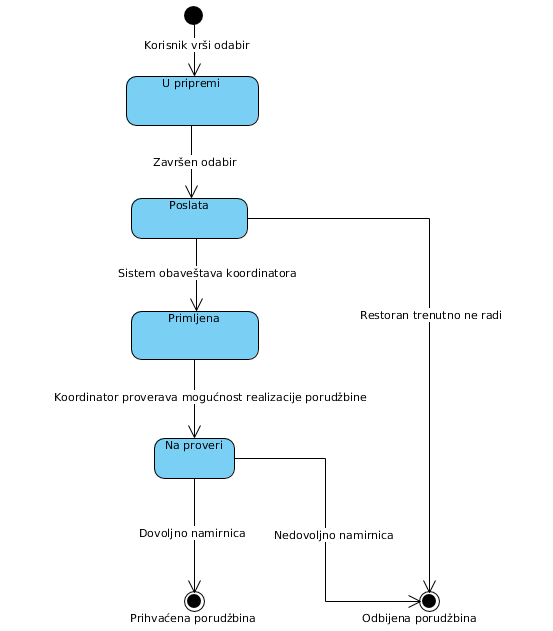
\includegraphics[width=136mm]{slike/Upravljanje_porudzbinom.png}\\


\subsubsection{Registracija korisnika na sajtu restorana}
\begin{itemize}
    \item \textbf{Kratak opis}:
    Korisnik prvi put pristupa sajtu i zato je neophodna registracija kako bi mogao poručiti hranu.
    \item \textbf{Učesnici}:
    Korisnik
    \item \textbf{Preduslovi}:
    Nema preduslova. 
    \item \textbf{Postuslovi}:
    Korisnik je registrovan. 
    \item \textbf{Glavni tok}:
   \begin{enumerate}
        \item Korisnik odlazi na vebsajt i otvara formu za registraciju
        \item Korisnik popunjava formu za registraciju
        \item Sistem vrši validaciju registracije
        \item Sistem beleži novog korisnika u bazi
        \item Sistem obaveštava korisnika o uspešnosti registracije
\end{enumerate}
\end{itemize}
\begin {itemize}
\item \textbf {Alternativni tokovi}: 
 3a: Korisnik nije uneo ispravne podatke za registraciju.\\
 Slučaj upotrebe se nastavlja na koraku 2.
 \end{itemize}
 \begin{itemize} 
     \item \textbf{Dodatne informacije}
 \begin{itemize}
     \item Neophodni podaci za registraciju korisnika su validna e-mail adresa, ime, prezime, adresa, korisničko ime i lozinka.
    \item Sistem validira novog korisnika tako što proverava da li već postoji nalog sa unetom e-mail adresom. Neophodno je i da korisničko ime bude jedinstveno.
 \end{itemize}
 \end{itemize}
 
 
\subsubsection{Onlajn naručivanje}
\begin{itemize}
    \item \textbf{Kratak opis}: Korisnik naručuje željenu hranu putem veb stranice. Porudžbina biva prihvaćena ili odbijena od strane koordinatora.
    \item \textbf{Učesnici}: Korisnik, koordinator.
    \item \textbf{Preduslovi}: Postojanje korisničkog naloga.
    \item \textbf{Postuslovi}: Prihvaćena, odnosno odbijena porudžbina.
    \item \textbf{Glavni tok}:
    
    1. Korisnik se prijavljuje na sajt restorana.\\
    2. Korisnik vrši odabir željenih proizvoda.\\
    3. Korisnik potvrđuje željenu porudžbinu klikom na dugme "Poruči".\\
    4. Sistem odbija porudžbinu u slučaju da restoran trenutno ne radi i obaveštava korisnika o tome.\\
    5. Sistem obaveštava koordinatora o prispeću zahteva.\\
    6. Koordinator proverava da li je moguće realizovati porudžbinu.\\
    7. Koordinator utvrđuje da svih namirnica potrebnih za datu porudžbinu ima u dovoljnim količinama.\\
    8. Koordinator prihvata porudžbinu klikom na dugme "Prihvati".\\
    9. Korisnik biva obavešten, od strane sistema, da je porudžbina prihvaćena.
    
     \item \textbf{Alternativni tokovi}:
     
     7. Koordinator utvrđuje da ne postoji dovoljna količina namirnica za pripremu porudžbine.\\
     8. Koordinator odbija porudžbinu klikom na dugme "Odbij".\\
     9. Korisnik biva obavešten, od strane sistema, da je porudžbina odbijena uz propratnu poruku.
    
\end{itemize}

\subsubsection{Naručivanje telefonom}
\begin{itemize}
    \item \textbf{Kratak opis}: Korisnik naručuje željenu hranu pozivom na telefon restorana. Porudžbina biva prihvaćena ili odbijena od strane koordinatora.
    \item \textbf{Učesnici}: Korisnik, koordinator.
    \item \textbf{Preduslovi}: Postojanje registrovanog telefonskog aparata u restoranu.
    \item \textbf{Postuslovi}: Prihvaćena, odnosno odbijena porudžbina.
     \item \textbf{Glavni tok}:
    
    1. Korisnik vrši poziv restorana.\\
    2. Korisnik vrši odabir željenih proizvoda.\\
    3. Koordinator proverava da li je moguće realizovati porudžbinu.\\
    4. Koordinator utvrđuje da svih namirnica potrebnih za datu porudžbinu ima u dovoljnim količinama.\\
    5. Koordinator prihvata porudžbinu i saopštava korisniku.\\
    6. Korisnik biva obavešten, od strane koordinatora, da je porudžbina prihvaćena.
    
    \item \textbf{Alternativni tokovi}:
     
     2. Korisnik biva obavešten, od strane telefonskog aprata, da restoran trenutno ne radi.\\
     4. Koordinator utvrđuje da ne postoji dovoljna količina namirnica za pripremu porudžbine.\\
     5. Koordinator odbija porudžbinu i saopštava korisniku.\\
     6. Korisnik biva obavešten, od strane koordinatora, da je porudžbina odbijena.
    
     
\end{itemize}


\subsection{Realizacija zahteva}
\subsubsection{Prosleđivanje porudžbine od koordinatora ka kuvaru}
\begin{itemize}
    \item \textbf{Kratak opis}:
    Koordinator prosledjuje zahtev za pripremu naručene hrane kuvaru.
    \item \textbf{Učesnici}:
    Koordinator, kuvar.
    \item \textbf{Preduslovi}:
    Postoje sve neophodne namirnice za pripremu poručenog jela.
    \item \textbf{Postuslovi}:
    Kuvar je primio zahtev za porudžbinom.
    \item \textbf{Glavni tok}:
   \begin{enumerate}
        \item Koordinator ostavlja cedulju sa naručenim jelom na glavni pult kuhinje.
        \item Kooordinator usmeno obaveštava kuvara da postoji nova porudžbina.
        \item Kuvar preuzima cedulju sa porudžbinom.
\end{enumerate}
\end{itemize}
 